\section{УРАВНЕНИЯ И НЕРАВЕНСТВА}
\subsection{Линейные уравнения с одной переменной}


\textbf{Важное замечание.} Большинство школьников считает, что линейное уравнение с одним неизвестным (одной переменной) всегда имеет один корень. На самом деле возможны три случая. Если уравнение приводится (после приведения подобных членов) к виду $ax=b,\enspace a\ne0$, то корень, в самом деле, единственный: $x=\frac{b}{a}$. Но если $a=0$, то возможны еще два случая. Если уравнение имеет вид  $0\cdot x=0$, то любое значение $x$ является корнем, т.е. уравнение имеет \textbf{бесконечное количество решений}.  Если же уравнение приводится к виду $0\cdot x=b,\enspace b\ne0$, то \textbf{решений нет}. В настоящем задачнике таких случаев, к сожалению, нет, но это не означает, что их не будет на экзамене. 

\textbf{Все}  задачи раздела  \textbf{1.3.1}  имеют единственное решение. Это явно предвзятая ситуация. Решать их все (а это ни много ни мало задачи  \textbf{583}-\textbf{769}) не имеет никакого смысла. Приведу решения нескольких задач. 

\textbf{583.}  $$6x+18=0;\quad6x=-18;\quad x=-3.$$ \newline \null \hspace*{\fill} Ответ: $-3$.     

\textbf{614.} $$-6x-5=4x;\quad -10x=5;\quad x=-0,5.$$ \newline \null \hspace*{\fill} Ответ: $-0,5$.  

\textbf{701.} $$x-\frac{x}{12}=-\frac{55}{12};\quad \frac{11}{12}x=-\frac{15}{12};\quad x=-5.$$ \newline \null \hspace*{\fill} Ответ: $-5$.   

\newpage \textbf{723.} $$\frac{x}{5}+\frac{x}{3}+x=\frac{23}{5};\quad x\left(\frac{1}{5}+\frac{1}{3}+1\right)=\frac{23}{5};\quad \frac{23}{15}=\frac{23}{5};\quad x=3.$$ \newline \null \hspace*{\fill} Ответ: $3$.    

\textbf{747.} $$\frac{5x-5}{3}-2x=2;\quad \frac{5}{3}x-2x=2+\frac{5}{3};\quad -\frac{1}{3}x=\frac{11}{3};\quad x=-11.$$ \newline \null \hspace*{\fill} Ответ: $-11$.    

\textbf{756.} $$\left(7-x\right)^2=\left(x+3\right)^2;\enspace 49-14x+x^2=x^2+6x+9;$$$$ -20x=-40;\enspace x=2.$$ \newline \null \hspace*{\fill} Ответ: $2$.    

\textbf{769.} $$\left(x-5\right)^2+\left(x+4\right)^2=2x^2;\enspace -10x+25+8x+16=0;$$$$ -2x=-41;\enspace x=20,5.$$ \newline \null \hspace*{\fill} Ответ: $20,5$.    

\subsection{Квадратные уравнения}


\textbf{770.} $$x^2-7x+10=0;\quad x_{1,2}=\frac{7\pm\sqrt{49-40}}{2}=\frac{7\pm3}{2}=\begin{cases}2 \\5 \end{cases}.$$ \newline \null \hspace*{\fill} Ответ: $2$.  

\newpage\textbf{775.} $$x^2-18=7x;\quad x^2-7-18=0;$$$$ x_{1,2}=\frac{7\pm\sqrt{49+72}}{2}=\frac{7\pm11}{2}=\begin{cases}-2 \\9 \end{cases}.$$ \newline \null \hspace*{\fill} Ответ: $9$. 

\textbf{778.} $$(-5x-3)(2x-1)=0;\enspace x_1=-\frac{3}{5}=-0,6;\enspace x_2=\frac{1}{2}=0,5.$$ \newline \null \hspace*{\fill} Ответ: $-0,6$. 

\textbf{779.} $$5x^2+20x=0,5x(x+4)=0;\quad x_1=0;\quad x_2=-4.$$ \newline \null \hspace*{\fill} Ответ: $-4$. 

\textbf{783.} $$-\frac{1}{5}x^2+20=0;\quad x^2=100;\quad x_{1,2}=\pm10.$$ \newline \null \hspace*{\fill} Ответ: $10$. 

\textbf{797.} $$x^2-24=-5x;\quad x^2+5x-24=0;$$$$ x_{1,2}=\frac{-5\pm\sqrt{25+96}}{2}=\frac{-5\pm11}{2}=\begin{cases}-8 \\3 \end{cases}.$$ \newline \null \hspace*{\fill} Ответ: $-8;\enspace3$. 

\textbf{805.} $$x^2-20x=-5-13-x^2;\quad 2x^2-15x+13=0;$$$$ x_{1,2}\frac{15\pm\sqrt{225-104}}{4}=\frac{15\pm11}{4}=\begin{cases}1 \\6,5 \end{cases}.$$ \newline \null \hspace*{\fill} Ответ: $1;\enspace6,5$. 

\textbf{814.} $$-3x^2-x+8=(x-3)^2;\quad -3x^2-x+8=x^2-6x+9;\quad 4x^2-5x+1=0;$$$$ x_{1,2}=\frac{5\pm\sqrt{25-16}}{8}=\frac{5\pm3}{8}=\begin{cases}0,25 \\1 \end{cases}.$$ \newline \null \hspace*{\fill} Ответ: $0,25;\enspace1$. 

\subsection{Рациональные уравнения}


\textbf{Важное предварительное замечание.} До сих пор мы имели дело только с линейными и квадратичными выражениями вида $ax+b$ или $ax^2+bx+c$. Эти выражения могут быть вычислены при \textbf{любом}  значении переменной $x$. Другими словами, \textbf{область допустимых значений} (ОДЗ)  переменной $-$ все действительные значения, $x\in R$ или $x\in (-\infty;\infty)$. Поэтому при решении линейных или квадратных уравнений мы и не задавались вопросом: входят найденные корни в ОДЗ или не входят. Все найденные корни являлись допустимыми.

В более сложных ситуациях (рациональные уравнения, логарифмические, показательные, тригонометрические уравнения (и не-\newline равенства) – это уже в 10-11 классах)  вопрос об ОДЗ  является \textbf{наиважнейшим}:  решив уравнение или неравенство, необходимо быть уверенным, что решения принадлежат ОДЗ. 
Нахождение ОДЗ тесно связано с тематикой решаемых задач. В рациональных выражениях ОДЗ определяется лишь требованием: если переменная содержится в знаменателе какого-либо выражения, \textbf{необходимо потребовать, чтобы этот знаменатель не обращался в ноль!} Справедливо золотое правило: прежде, чем решать задачу, следует найти ОДЗ, т.е. ту область значений переменной $x$, в которой поставленная задача имеет смысл.
И еще один момент. Можно выписать неравенство (или несколько неравенств), определяющие ОДЗ. Но совсем не обязательно решать эти неравенства: достаточно \textbf{проверить}, удовлетворяют ли найденные решения этим неравенствам. Когда корень один (или несколько), сделать это обычно несложно. Если же, например, решается неравенство, и решениями могут быть целые интервалы значений $x$, то существуют специальные графические приемы получения окончательного вердикта. Об этом будет разговор в свое время.

\textbf{817.}  Сначала найдем ОДЗ: $x-2\ne0;\enspace x\ne2$. Затем  решаем уравнение: $$\frac{11}{x-2}=\frac{11}{2};\quad x-2=2;\quad x=4$$ (входит в ОДЗ). \newline \null \hspace*{\fill} Ответ: $4$.

Часто случается так, что найденный корень (корни) входят в ОДЗ. Очень велик процент ошибок в школьных работах,  связанных  с пренебрежительным отношением к ОДЗ. Лучше всего приобрести \textbf{полезную} привычку: если в начале решения была найдена ОДЗ, то в конце работы следует написать фразу: «Найденный корень (корни) входит в ОДЗ».  

\textbf{827.} ОДЗ: $$\begin{cases} x\ne 14 \\ x\ne 7\end{cases}.$$$$\frac{7}{x-14}=\frac{14}{x-7};\enspace \frac{1}{x-14}=\frac{2}{x-7};$$$$ x-7=2x-28;\enspace x=21\text{(входит в ОДЗ).}$$ \newline \null \hspace*{\fill} Ответ: $21$.

\textbf{832.} ОДЗ: $$\begin{cases} x\ne -6 \\ x\ne 1\end{cases}.$$ $$\frac{1}{x+6}+\frac{1}{x-1}=0;\enspace x-1+x+6=0;\enspace 2x=-5;$$$$ x=-2,5\text{(входит в ОДЗ)}.$$
\newline \null \hspace*{\fill} Ответ: $-2,5$.

\newpage\textbf{841.} ОДЗ: $x\ne15$. $$\frac{x-5}{x-15}=-1;\enspace x-5=-x+15;\enspace 2x=20;\enspace x=10\text{(входит в ОДЗ)}.$$ \newline \null \hspace*{\fill} Ответ: $10$.

\textbf{851.} ОДЗ: $x\ne0$.$$x-\frac{12}{x}=1;\enspace x^2-x-12=0;\enspace x_{1,2}=\frac{1\pm7}{2}=\begin{cases} -3 \\ 4 \end{cases}\text{(входит в ОДЗ)}.$$ \newline \null \hspace*{\fill} Ответ: $-3;\enspace 4$.

Кстати говоря. Иногда школьники допускают досадную ошибку: неправильно вычисляют корни квадратного уравнения. Существует простейшая проверка корней по теореме Виета: произведение корней равно свободному члену уравнения, а сумма корней $-$ коэффициенту при $x$ с обратным знаком (это только в том случае, если коэффициент при $x^2$  равен 1). Проверка (устная, разумеется) занимает несколько секунд, а ошибка стоит гораздо дороже. 

\textbf{858.} ОДЗ: $x\ne-2$. $$\frac{x^2+4x+3}{x+2}=0;\enspace x^2+4x+3=0$$$$ x_{1,2}=-2\pm \sqrt{4-3}=-2\pm1=\begin{cases} -3 \\ -1 \end{cases}.$$
		
Оба корня входят в ОДЗ. \newline \null \hspace*{\fill} Ответ: $-3;\enspace -1$.

Для нахождения корней квадратного уравнения использована формула для случая четного коэффициента  при $x$. 


\subsection{Системы двух уравнений с двумя переменными}


Если знаменатели всех выражений не содержат переменных $x,y$, то ОДЗ системы имеет вид $x\in R,\enspace y\in R$ и эти неравенства не выписывают и никаких проверок не делают. В более сложных ситуациях выписывание неравенств, определяющих ОДЗ системы, и проверка $-$ непременный атрибут решения!  

\textbf{864.}  Школьники должны уметь решать систему двух линейных уравнений с двумя неизвестными  двумя способами.

1. Одно из уравнений используется для того, чтобы выразить  одну из неизвестных через другую. Это соотношение подставляют в другое уравнение, получают одно линейное уравнение с одной неизвестной и решают его. Найденная вначале связь между неизвестными используется затем для нахождения другой неизвестной.

2. Уравнения системы можно сложить или вычесть одно из другого, предварительно умножив их на удобные числа (отличные от нуля). Такой прием позволяет исключить одну из неизвестных, решить уравнение относительно оставшейся неизвестной, а затем из любого из уравнений найти вторую неизвестную. Такая процедура  корректна и не изменяет множества решений системы. 

В нашем случае удобно умножить второе уравнение на $2$ и сложить его с первым. Тем самым из системы исключается $y$, а уравнение для $x$ принимает вид: $-x=0$, откуда получаем $x=0$. Теперь, например, из второго уравнения получаем: $-2y=2;\enspace y=-1$. Ответ принято записывать в скобках, сначала $x$, затем $y$. \newline \null \hspace*{\fill} Ответ: $(0;-1)$. 

\textbf{865.}  $$\begin{cases} 4x-2y=-9 \\ 3x-3y=-6 \end{cases}$$ Из второго уравнения $x=y-2$, тогда первое принимает вид: $4(y-2)-2y=-9$ откуда $y=-0,5$. Соответственно $x=y-2=-2,5.$ \newline \null \hspace*{\fill} Ответ: $(-2,5;-0,5)$.             

\newpage \textbf{868.} Решение можно оформить и так:
$$\begin{cases} 4x+y=-3 \\ -y-x^2=6 \end{cases},\enspace\begin{cases} y=-4x-3 \\ 4x+3-x^2=6 \end{cases},\enspace \begin{cases} y=-4x-3 \\ x^2-4x+3=0 \end{cases}.$$ $$x_{1,2}=2\pm1=\begin{cases}1 \\ 3 \end{cases}.\enspace y_{1,2}=\begin{cases}-7 \\ -15 \end{cases}.$$ \newline \null \hspace*{\fill} Ответ: $(1;-7);\enspace(3;-15)$.

\textbf{872.}  $$\begin{cases}x+y=2\\ xy=-15 \end{cases}.$$ Эту систему можно решить обычным способом: выразить  из первого уравнения $x$ через $y$, подставить это выражение во второе, получить квадратное уравнение относительно $y$ и т.д. 

Есть еще один изящный прием, основанный на следующих двух соображениях.  

1. Эта система симметричная, т.е. замена $x$ на $y$ и обратно не изменяет ее вида. Это означает, что если $(\alpha;\beta)-$ решение системы, то и $(\beta;\alpha)$ является ее решением. 

2. Поскольку задана сумма и произведение неизвестных, то в соответствии с теоремой Виета можно утверждать, что $x$ и $y$ являются корнями одного и того же квадратного уравнения  \newline$z^2-2z-15=0$. Решив это уравнение, получим  $$z_{1,2}=1\pm4=\begin{cases}-3\\ 5 \end{cases}.$$ Это позволяет сразу записать ответ. \newline \null \hspace*{\fill} Ответ: $(-3;5);\enspace(5;-3)$.  

\textbf{874.}  $$\begin{cases}-x+y=3\\ xy=10 \end{cases},\enspace \begin{cases}-x+y=3\\ (-x)y=-10 \end{cases}.$$ Здесь предыдущий прием можно немного модифицировать: считаем что система симметрична относительно переменных $-x$ и  $y$, которые являются корнями одного и того же уравнения \newline$z^2-3z-10=0$. Решим его  $$z_{1,2}=\frac{3\pm7}{2}=\begin{cases}-2\\ 5 \end{cases}$$ и запишем ответ (только не забудем, что мы получили корни для неизвестных $-x$ и $y$). \newline \null \hspace*{\fill} Ответ: $(2;5);\enspace(-5;2)$. 

\textbf{878.} $$\begin{cases}-x+y=7\\ x^2+y^2=25 \end{cases},\enspace \begin{cases}y=7+x\\ x^2+49+14x+x^2=25 \end{cases},\enspace $$$$\begin{cases}y=7+x\\ x^2+7x+12=0 \end{cases}.x_{1,2}=\frac{-7\pm1}{2}=\begin{cases}-4\\-3 \end{cases}.\enspace y_{1,2}=\begin{cases}3\\4 \end{cases}$$ \newline \null \hspace*{\fill} Ответ: $(-4;3);\enspace(-3;4)$.


\subsection{Числовые неравенства и их свойства}


\textbf{Важное замечание.} Неравенства и их свойства $-$ это очень серьезный раздел математики. Школьники допускают громадное количество ошибок, решая неравенства. Поэтому необходимо очень тщательно разобраться в теории и методах решения неравенств. Особое внимание следует уделить геометрической трактовке на числовой оси.

\textbf{880.} Если $a>b$, то на числовой оси точка $a$ находится правее точки $b$. Но тогда  справедливо и более сильное неравенство $a>\linebreak>b-c$, где $c-$ любое неотрицательное число ($c\geq0$). Этому условию удовлетворяет  только вариант ответа 4). \newline \null \hspace*{\fill} Ответ: $4$.

\textbf{881.} В варианте ответа 3) неравенство приводится к виду $a>\linebreak>2b-2$. Среди приведенных ответов только это неравенство справедливо при  любых $a>2b$. \newline \null \hspace*{\fill} Ответ: $3$.

\textbf{883.} Неравенство $-a>-b$ эквивалентно (равносильно) неравенству $b>a$. Из приведенных ответов  более сильным является только неравенство 2), которое приводится к виду $b>a-1$. \newline \null \hspace*{\fill} Ответ: $2$. 

\textbf{885.} Только неравенство 3) приводится к виду $a>c$, которое противоречит условию $a<c$. \newline \null \hspace*{\fill} Ответ: $3$. 

\textbf{889.} Аналогичная задача. \newline \null \hspace*{\fill} Ответ: $4$. 

\textbf{890.} Из приведенного рисунка ясно, что $a>c$. Этому условию противоречит только вариант ответа 1). \newline \null \hspace*{\fill} Ответ: $1$. 

\textbf{895.} Из приведенного рисунка видно, что $3<a<4$. Подстановкой в предлагаемые неравенства легко убедиться, что справедливо только неравенство 1). \newline \null \hspace*{\fill} Ответ: $1$.

\textbf{897.} Аналогичная задача. \newline \null \hspace*{\fill} Ответ: $1$. 

\textbf{900.} Т.к. $1<a<2$, то несложно определить интервалы, в которых расположены заданные числа.  

Напомню, что к обеим частям  неравенства можно \textbf{прибавить} любое (положительное или отрицательное) число. Если неравенство двойное (у которого три части: левая, средняя и правая), то любое число можно прибавить ко всем трем частям неравенства. Из этих соображений $0<a-1<1$.

При умножении всех частей неравенства на отрицательное число знаки неравенств \textbf{изменяются на противоположные}. Поэтому $-2<-a<-1$.     
Наконец, если в двойном неравенстве левая и правая части \textbf{положительны}, то при замене всех трех выражений на обратные знаки неравенств также  \textbf{изменяются на противоположные}. Следовательно, можно записать $\frac{1}{2}<\frac{1}{a}<1$. Умножив это неравенство на $-1$, получим $-1<-\frac{1}{a}<\frac{1}{2}$.

Сравнивая полученные интервалы, убеждаемся, что  в порядке убывания заданные числа расположены в варианте  3). \newline \null \hspace*{\fill} Ответ: $3$. 

\newpage \textbf{902.} В нашем случае $-2<a-1$, т.е. $1<-a<2$ и $\frac{1}{2}<-\frac{1}{a}<1$. В тоже время, если неравенство $-a>1$ умножить на положительное число $-a$, то получим $a^2>-a$. Таким образом, в порядке убывания заданные числа располагаются в варианте 1). \newline \null \hspace*{\fill} Ответ: $1$.

\textbf{Замечание.} Можно, видимо, такие задачи решать проще,  «на глазок», ориентируясь на \textbf{остроту своего зрения}. Например, в данной задаче $a\approx1,3$. Но тогда $-a\approx1,3;\enspace a^2\approx 1,69;\enspace -\frac{1}{a}\approx\linebreak\approx\frac{1}{1,3}\approx0,77$. Если в задаче требуется из трех ответов только указать верный, то нет проблем:  числа $1,69;\enspace1,3;\enspace0,77$ достаточно сильно различаются, чтобы быть уверенным в результате.

\textbf{907.} Классическое решение. Т.к. $-a<a<-1$, то $1<-a<2$, т.е. $-a>a$. Т.к. $-a>1$, то $-a\cdot a<a;\enspace -a^2<a$ (при умножении неравенства на отрицательное число знак неравенства изменяется на противоположный). Таким образом, $-a^2<a<-a$. \newline \null \hspace*{\fill} Ответ: $4$.

Решение «на глазок». $a\approx-1,3;\enspace -a\approx1,3;\enspace -a^2\approx-1,69.\enspace -a^2<\linebreak<a<-a.$

\textbf{908.} Неправильным является только утверждение 2), т.к. $x$ и $y$ имеют разные знаки. Остальные утверждения верны (с учетом того, что $|x|>|y|$ и $y<0$). \newline \null \hspace*{\fill} Ответ: $2$.

\textbf{911.} Т.к. $a<0,\enspace b>0,\enspace c<0$, то $abc>0$, первое неравенство верное. 

Т.к. $|b|<|c|$, второе неравенство неверное. 

Если даны два неравенства одного знака с \textbf{положительными членами} $d>e,\enspace f>g$, то их можно почленно перемножить: $df>eg$. Т.к. $-a<1$, то $-\frac{1}{a}>1$, а поскольку $-c>1$, то перемножая два последних неравенства, получаем  $\frac{c}{a}>1>b$. Третье неравенство верное. Четвертое неравенство также верное. Неверным оказывается только неравенство 2). \newline \null \hspace*{\fill} Ответ: $2$.

Легко убедиться, что решение «на глазок» ($c\approx-1,5;\enspace a\approx-0,5;\linebreak v\approx0,5$) очень быстро приводит к тому же результату.


\subsection{Линейные неравенства с одной переменной}

\textbf{915.} $$-3-3x>7x-9;\enspace -10x>-6;\enspace x<0,6;\enspace x\in(-\infty;0,6).$$ \newline \null \hspace*{\fill} Ответ: $4$. 

\textbf{921.} $$7x+9\leq9x-8;\enspace -2x\leq-17;\enspace x\geq8,5;\enspace x\in[8,5;\infty).$$ \newline \null \hspace*{\fill} Ответ: $3$. 

\textbf{930.} $$4x+5\geq6x-2;\enspace-2x\geq-17;\enspace x\leq3,5;\enspace x\in(-\infty;3,5].$$ \newline \null \hspace*{\fill} Ответ: $2$. 

\textbf{934.} $$3-2(x-3)>18-5x;\enspace 3x>9;\enspace x>3;\enspace x\in(3;\infty).$$ \newline \null \hspace*{\fill} Ответ: $4$.

\textbf{938.} $$4-7(x+3)\leq-9;\enspace -7x\leq8;\enspace x\geq-\frac{8}{7};\enspace x\in\bigg[-\frac{8}{7};\infty\bigg).$$ \newline \null \hspace*{\fill} Ответ: $3$. 

\textbf{939.} $$6x-7>7x+8;\enspace -x>15;\enspace x<-15;\enspace x\in(-\infty;-15).$$ \newline \null \hspace*{\fill} Ответ: $4$.

\textbf{945.} $$4a+9<0;\enspace 4a<-9;\enspace a<-\frac{9}{4};\enspace a\in\bigg(-\infty;\frac{9}{4}\bigg).$$  \newline \null \hspace*{\fill} Ответ:  1.

\textbf{955.} $$-3x+9<0;\enspace -3x<-9;\enspace x>3;\enspace x\in (2;\infty).$$ \newline \null \hspace*{\fill} Ответ: $(3;\infty)$.

Задачи  \textbf{956}-\textbf{1118} элементарны.


\subsection{Системы линейных неравенств с одной переменной}


\textbf{1119.} Чтобы решить систему неравенств, надо сначала решить каждое  неравенство системы, а затем объединить полученные решения (найти \textbf{пересечение} множеств решений отдельных $\newline$ неравенств).  Объединяют решения обычно графически. $$\begin{cases}x>4\\-3x\leq3 \end{cases}, \begin{cases}x>4\\x\geq-1 \end{cases}$$
\begin{figure}[h]
	\center{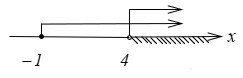
\includegraphics[width=0.4\linewidth]{Algebra/1.3.7/1}}
\end{figure}
\newline \null \hspace*{\fill} Ответ: $(4;\infty)$. 

1123. $$\begin{cases}x>4,3\geq0\\x+5\leq 10 \end{cases},\quad\begin{cases}x\geq4,3\\x\leq5 \end{cases},\quad 4,3\leq x\leq5.$$    

\begin{figure}[h!]
	\center{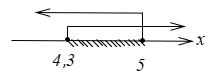
\includegraphics[width=0.4\linewidth]{Algebra/1.3.7/2}}
\end{figure}

\null \hspace*{\fill} Ответ: $4$. 

1126. $$\begin{cases}x<9\\8-x>0 \end{cases},\quad\begin{cases}x<9\\x<8 \end{cases},\quad x<8.$$                 

\begin{figure}[h!]
	\center{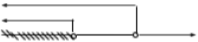
\includegraphics[width=0.4\linewidth]{Algebra/1.3.7/3}}
\end{figure}

\null \hspace*{\fill} Ответ: $2$. 

1129. $$\begin{cases}x>-1\\-4-x>0 \end{cases},\quad\begin{cases}x>-1\\x<-4 \end{cases},\quad x<\varnothing.$$                 
                 

Символ $\varnothing$ используется для обозначения пустого множества.$\newline$ Множество решений пусто: система не имеет решений. Неравенства противоречат друг другу. На графической диаграмме нет заштрихованной области.

\begin{figure}[h!]
	\center{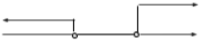
\includegraphics[width=0.4\linewidth]{Algebra/1.3.7/4}}
\end{figure}

\null \hspace*{\fill} Ответ: $4$. 

\subsection{Квадратные неравенства}


Квадратные неравенства решаются графически. Изображается парабола $-$ график квадратного трехчлена. Важно правильно изобразить вершину параболы (где она находится: выше оси $x$, ниже или на самой оси?), как направлены ветви параболы (вниз или вверх), как  расположены корн квадратного трехчлена на оси $x$). Затем на числовой оси с учетом знака неравенства наносится штриховка. Ось ординат на таком графике не наносится.

\newpage \textbf{1134.} $$x^2>9;\quad x^2-9>0$$      

\begin{figure}[h!]
	\center{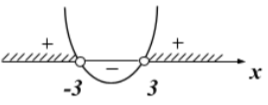
\includegraphics[width=0.4\linewidth]{Algebra/1.3.8/1}}
\end{figure}

\null \hspace*{\fill} Ответ: $4$.  

\textbf{1144.} \newline \null \hspace*{\fill} Ответ: $3$. 

\textbf{1149.} Чтобы уверенно отвечать на такие вопросы, нужна хорошая практика решения квадратных неравенств и построения графиков парабол. Особое внимание надо уделять корням квадратного трехчлена. Следует их помечать выколотыми точками (незакрашенными кружочками),  если знак неравенств строгий ($<$ или $>$) и «жирными» точками (закрашенными кружочками), если знак нестрогий ($\leq$ или $\geq$). Соответственно, корни затем не войдут или войдут в множество решений, а в изображении множества решений (в ответе) будут использоваться круглые  или квадратные скобки.

В нашей конкретной задаче изображение решения соответствует неравенству 2), т.к. для этого варианта  ветви параболы направлены вверх, квадратный трехчлен принимает неотрицательные выражения \textbf{вне} промежутка между корнями $x_1=0$ и $x_2=3$, а сами корни (помеченные на рисунке «жирными» точками), \textbf{входят} в множество решений, т.к. знак неравенства \textbf{нестрогий}. Всем приведенным словам соответствует график:

\begin{figure}[h!]
	\center{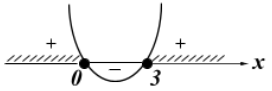
\includegraphics[width=0.4\linewidth]{Algebra/1.3.8/2}}
\end{figure}

\null \hspace*{\fill} Ответ: $2$.

\newpage \textbf{1154.} $$3x-x^2\leq0$$

\begin{figure}[h!]
	\center{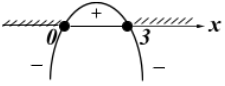
\includegraphics[width=0.4\linewidth]{Algebra/1.3.8/3}}
\end{figure}

\null \hspace*{\fill} Ответ: $2$.          

Вообще говоря, можно любое квадратное неравенство привести к такому виду, что квадратный трехчлен в левой части имеет положительный коэффициент при $x^2$ (если это не так, надо умножить все члены на $-1$ и сменить знак неравенства на противоположный). Тогда на всех графических рисунках ветви параболы направлены вверх. Разумеется, окончательный ответ при этом не изменяется.  

\textbf{1159.} $$x^2+9x+20<0;\quad x\in (-5;-4).$$
Корни: $$x_{1,2}=\frac{-9\pm1}{2}=\begin{cases}-5\\-4 \end{cases}$$

\begin{figure}[h!]
	\center{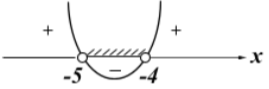
\includegraphics[width=0.4\linewidth]{Algebra/1.3.8/4}}
\end{figure}

\null \hspace*{\fill} Ответ: $2$.   

\textbf{1164.}  Варианты ответов 1) и 3) можно исключить сразу (если ветви параболы направлены вверх, то обязательно найдутся значения $x$, при которых парабола принимает положительные значения). В вариантах 2) и 4) ветви также направлены вверх. \newpage Отрицательных решений не будет, если график полностью располагается \textbf{над} осью $x$, т.е. если он имеет вид, изображенный ниже на схематическом рисунке. 

\begin{figure}[h!]
	\center{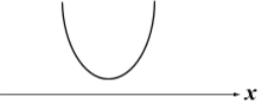
\includegraphics[width=0.4\linewidth]{Algebra/1.3.8/5}}
\end{figure}

Для этого необходимо, чтобы соответствующий квадратный трехчлен не имел корней, т.е. его дискриминант был отрицательным. Легко убедиться, что это выполняется только для варианта 4). \newline \null \hspace*{\fill} Ответ: $4$.    

Задачи \textbf{1165}-\textbf{1168} решаются аналогично.

\textbf{1169.}  Только в варианте 4) неравенство справедливо при $x\in R$, в остальных случаях это не так. Схематически график имеет такой же вид, как в задаче \textbf{1164}. \newline \null \hspace*{\fill} Ответ: $4$. 

Все остальные задачи данного раздела решаются стандартным образом: все члены переносятся в левую часть, приводятся подобные члены (если потребуется), находятся корни (иногда они видны невооруженным взглядом, как, например, в задачах \textbf{1174}-\textbf{1178}). Затем строится график и в соответствии со знаком неравенства наносится штриховка. Еще раз: требуется особое внимание к корням квадратного трехчлена. 

\textbf{1174.} $$(x-4)(x-6)>0$$                 

\begin{figure}[h!]
	\center{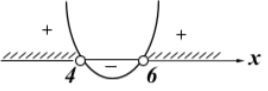
\includegraphics[width=0.4\linewidth]{Algebra/1.3.8/6}}
\end{figure}

\null \hspace*{\fill} Ответ: $x\in(-\infty;4)\cup(6;\infty)$.

Значок $\cup$ обозначает объединение множеств: $x$ принадлежит множеству $(-\infty;4)$ или множеству $(6;\infty)$.
 
\textbf{1188.} $$x^2+3x\leq28;\quad x^2+3x-28\leq0;\quad (x+7)(x-4)\leq0$$ 

\begin{figure}[h!]
	\center{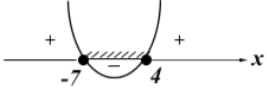
\includegraphics[width=0.4\linewidth]{Algebra/1.3.8/7}}
\end{figure}

\null \hspace*{\fill} Ответ: $x\in[-7;4]$. 

\textbf{1203.} $$x^2\geq7x+8;\quad x^2-7x-8\geq0;\quad (x+1)(x-8)\geq0$$

\begin{figure}[h!]
	\center{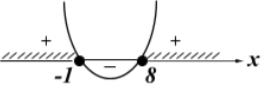
\includegraphics[width=0.4\linewidth]{Algebra/1.3.8/8}}
\end{figure}

\null \hspace*{\fill}Ответ: $x\in(-\infty;-1]\cup[8;\infty).$

\textbf{1206.} $$x^2-7x<6x-15x^2;\quad 2x^2-13+15<0;\quad 2(x-1,5)(x-5)<0$$

\begin{figure}[h!]
	\center{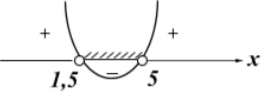
\includegraphics[width=0.4\linewidth]{Algebra/1.3.8/9}}
\end{figure}

\null \hspace*{\fill} Ответ: $x\in(1,5;5)$.

\newpage \textbf{1218.} $$10x^2-24x+16\leq 5x^2;\quad 5x^2-24x+16\leq 0;\quad 5(x-0,8)(x-4)\leq0$$

\begin{figure}[h!]
	\center{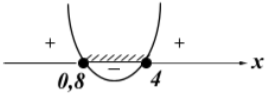
\includegraphics[width=0.4\linewidth]{Algebra/1.3.8/10}}
\end{figure}

\null \hspace*{\fill} Ответ: $x\in[0,8;4]$. 

\textbf{1234.} $$x^2-13x+45\leq 6x^2-16x+19;\quad 5x^2-3x-26\geq0;$$ $$ 5(x+2)(x-2,6)\geq0$$

\begin{figure}[h!]
	\center{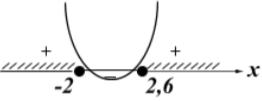
\includegraphics[width=0.4\linewidth]{Algebra/1.3.8/11}}
\end{figure}

\null \hspace*{\fill} Ответ: $x\in(-\infty;-2]\cup[2,6;\infty)$. 

\textbf{1261.} $$-3x^2+3x+22\leq(x-3)^2;\quad 4x^2-9x-13\geq0;\quad(x+1)(x-3,25)\geq0$$

\begin{figure}[h!]
	\center{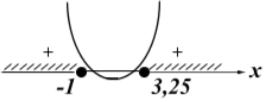
\includegraphics[width=0.4\linewidth]{Algebra/1.3.8/12}}
\end{figure}

\null \hspace*{\fill} Ответ: $x\in(-\infty;-1]\cup[3,25;\infty)$. 